\section{84 -- Largest Rectangle in Histogram}
Given $n$ non-negative integers representing the histogram's bar height where the width of each bar is 1, find the area of largest rectangle in the histogram.
\begin{figure}[H]
\begin{tikzpicture}
\draw (0,0) rectangle ++(1,2);
\draw (1,0) rectangle ++(1,1);
\draw (2,0) rectangle ++(1,5);
\draw (3,0) rectangle ++(1,6);
\draw (4,0) rectangle ++(1,2);
\draw (5,0) rectangle ++(1,3);
\node at (0.5,2.3) {2};
\node at (1.5,1.3) {1};
\node at (2.5,5.3) {5};
\node at (3.5,6.3) {6};
\node at (4.5,2.3) {2};
\node at (5.5,3.3) {3};
\end{tikzpicture}
\end{figure}
Above is a histogram where width of each bar is 1, given height $H = (2,1,5,6,2,3)$.
\begin{figure}[H]
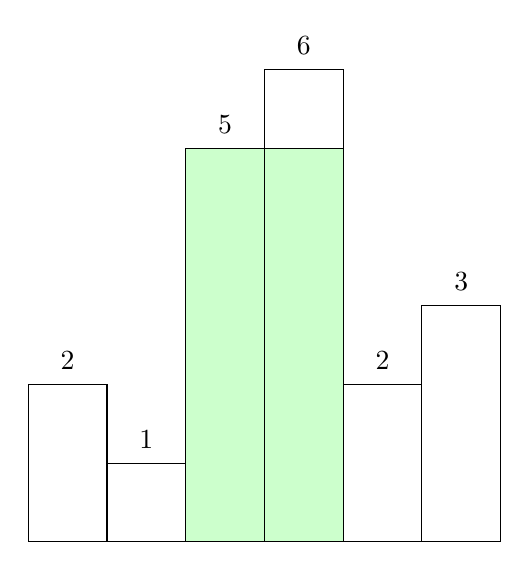
\begin{tikzpicture}

\draw (0,0) rectangle ++(1,2);
\draw (1,0) rectangle ++(1,1);
\fill[green!20!white] (2,0) rectangle ++(2,5);
\draw (2,0) rectangle ++(1,5);
\draw (3,0) rectangle ++(1,5);
\draw (3,0) rectangle ++(1,6);
\draw (4,0) rectangle ++(1,2);
\draw (5,0) rectangle ++(1,3);
\node at (0.5,2.3) {2};
\node at (1.5,1.3) {1};
\node at (2.5,5.3) {5};
\node at (3.5,6.3) {6};
\node at (4.5,2.3) {2};
\node at (5.5,3.3) {3};
\end{tikzpicture}
\end{figure}
The largest rectangle is shown in the light green area, which has area $A= 10$ unit.
\subsection{Stack Based Approach}
直方图中每个bar的宽度是1,对于每一个bar $x$, 需要计算出以$x$的高度作为最小高度所围起来的矩形的面积。那么如何计算出这样的面积呢?我们需要找到在$x$左边 找到第一个高度小于$x$高度的bar的index $\alpha$,同时在$x$右边找到第一个高度小于$x$高度的bar的index $\beta$。

从左到右遍历直方图高度数组 $H$,同时maintain一个ascending stack $S$。 Ascending means the bar at top index of the stack has maximum height so far.

When we are traversing at index $i$, and the bar at index $i$ is \textbf{shorter} than the bar at top of the stack, we will pop out each index in the stack. Apparently, the bar at index $i$ is the $\beta$ of each popped bar (i.e. $\beta=i$).

Each time we pop a bar index, we check current index at the top of the stack, say $t$. Now the bar at index $t$ will be the $\alpha$ of the popped bar (i.e., $\alpha=t$). 

we will calculate the area of the rectangle that is formed by the popped bar spanning from $\alpha+1$ to $\beta-1$ and update the maximum area so far.

There is a edge case: When we pop a bar index, if stack become empty, this means all the bar on the left side of the popped bar are all higher than 
that popped one (We can think of $\alpha=-1$)

\setcounter{lstlisting}{0}
\begin{lstlisting}[style=customc, caption={Stack}]
int largestRectangleArea( vector<int>& heights )
{
    int n = static_cast<int>( heights.size() );
    stack<int> stk;
    int ans = 0;
    for( int i = 0; i < n; ++i )
    {
        while( !stk.empty() && ( heights[stk.top()] >= heights[i] ) )
        {
            //beta is i
            int h = heights[stk.top()];
            stk.pop();
            //alpha will be current top of stk
            //or -1 if stk is empty
            int alpha = stk.empty() ? -1 : stk.top();
            //the rectange is spanning from (alpha+1) to (i-1)
            int w = ( i - 1 ) - ( alpha + 1 ) + 1;
            int area = h * w;
            //update maximum area so far
            ans = ( max )( area, ans );
        }
        stk.push( i );
    }
    //when traversing is completed
    //we may still have bars in the stack
    //because last bar is higher
    while( !stk.empty() )
    {
        //beta is n
        int h = heights[stk.top()];
        stk.pop();
        //alpha will be current top of stk
        //or -1 if stk is empty
        int alpha = stk.empty() ? -1 : stk.top();
        //the rectange is spanning from (alpha+1) to (n-1)
        int w = n - 1 - ( alpha + 1 ) + 1;
        int area = h * w;
        //update maximum area so far
        ans = ( max )( area, ans );
    }
    return ans;
}
\end{lstlisting}
